\documentclass[11pt]{article}
\usepackage[margin=1in]{geometry}
\usepackage{booktabs}
\usepackage{xcolor}
\usepackage{amsmath}
\usepackage{float}
\usepackage{graphicx}
\usepackage{hyperref}
\hypersetup{colorlinks=true, linkcolor=blue!60!black}

\newcommand{\win}[1]{\textcolor{green!50!black}{\textbf{#1}}}
\newcommand{\bad}[1]{\textcolor{red!70!black}{#1}}

\title{Routing Evaluation --- No Interference}
\author{Autonomous Networks Research Group (ANRG)\\University of Southern California}
\date{}
\begin{document}
\maketitle
\tableofcontents
\newpage

\section{Evaluation Setup}

Identical workloads and scheduler/routing combinations as the \texttt{csma\_bianchi}
interference evaluations, but with \texttt{--interference none}: links share
bandwidth fairly under concurrent flows but there is no inter-link interference.
Results can be compared directly against the interference reports to isolate
the cost imposed by wireless contention.

\begin{table}[H]\centering
\begin{tabular}{ll}\toprule
\textbf{Parameter} & \textbf{Value} \\\midrule
Interference & \textbf{none} (intra-link fair-share only) \\
Schedulers & HEFT (calibrated), HEFT-1, HEFT-2 \\
Grid routing & W, S, SH, GS, GC, GB, GO, GSD, GSD-D \\
Random routing & W, S, SH, GO, GS, GSD, GSD-D \\
Seeds per combo & 30 \\
Grid sizes & $4\times4$ (16 nodes, 40\,m spacing) and $7\times7$ (49 nodes) \\
Random nodes & 50, uniform in $[0,L]^2$, comm range $R=80$\,m \\
Density levels & L150--L500 ($L=150$\,m to $500$\,m) \\
DAGs & Small (8 tasks, fork-join), Large (30/60 tasks, pipeline) \\
\bottomrule\end{tabular}
\caption{Evaluation parameters. All other settings identical to the interference reports.}
\end{table}

Error bars and uncertainty columns report 95\,\% confidence intervals
($t_{29}=2.045$, $n=30$ seeds): $\mathrm{CI} = 2.045 \cdot \sigma / \sqrt{30}$.

\section{Grid Network Results}

Mean makespan and additional metrics averaged over 30 seeds.
\win{Bold green}: overall experiment winner. \bad{Red}: worst in that scheduler column.

\subsection{$4\times4$ Grid, Small (8 tasks, fork-join)}

\begin{table}[H]\centering\small
\begin{tabular}{l r@{$\pm$}l r@{$\pm$}l r@{$\pm$}l}
\toprule
\textbf{Routing} & \multicolumn{2}{c}{\textbf{HEFT (s)}} & \multicolumn{2}{c}{\textbf{HEFT-1 (s)}} & \multicolumn{2}{c}{\textbf{HEFT-2 (s)}} \\
\midrule
  W & \win{13.500} & 0.000 & \win{13.500} & 0.000 & \win{13.500} & 0.000 \\
  S & \win{13.500} & 0.000 & \win{13.500} & 0.000 & \win{13.500} & 0.000 \\
  SH & \win{13.500} & 0.000 & \win{13.500} & 0.000 & \win{13.500} & 0.000 \\
  GS & \win{13.500} & 0.000 & \win{13.500} & 0.000 & \win{13.500} & 0.000 \\
  GC & \win{13.500} & 0.000 & \win{13.500} & 0.000 & \win{13.500} & 0.000 \\
  GB & \win{13.500} & 0.000 & \win{13.500} & 0.000 & \win{13.500} & 0.000 \\
  GO & \win{13.500} & 0.000 & \win{13.500} & 0.000 & \win{13.500} & 0.000 \\
  GSD & \win{13.500} & 0.000 & \win{13.500} & 0.000 & \win{13.500} & 0.000 \\
  GSD-D & \win{13.500} & 0.000 & \win{13.500} & 0.000 & \win{13.500} & 0.000 \\
\midrule
  \textit{Best} & \textit{W 13.500} & --- & \textit{W 13.500} & --- & \textit{W 13.500} & --- \\
\bottomrule\end{tabular}
\caption{$4\times4$ small (8 tasks, fork-join) --- mean$\pm$95\,\%\,CI makespan (s) over 30 seeds.}
\end{table}

\begin{table}[H]\centering\small
\begin{tabular}{l r r r r r r r r r}
\toprule
\textbf{Routing} & \multicolumn{3}{c}{\textbf{HEFT}} & \multicolumn{3}{c}{\textbf{HEFT-1}} & \multicolumn{3}{c}{\textbf{HEFT-2}} \\
\cmidrule(lr){2-4}\cmidrule(lr){5-7}\cmidrule(lr){8-10}
& \textbf{Hops} & \textbf{P-LU} & \textbf{XD(s)} & \textbf{Hops} & \textbf{P-LU} & \textbf{XD(s)} & \textbf{Hops} & \textbf{P-LU} & \textbf{XD(s)} \\
\midrule
  W & 0.0 & 0.000 & 0.0 & 0.0 & 0.000 & 0.0 & 0.0 & 0.000 & 0.0 \\
  S & 0.0 & 0.000 & 0.0 & 0.0 & 0.000 & 0.0 & 0.0 & 0.000 & 0.0 \\
  SH & 0.0 & 0.000 & 0.0 & 0.0 & 0.000 & 0.0 & 0.0 & 0.000 & 0.0 \\
  GS & 0.0 & 0.000 & 0.0 & 0.0 & 0.000 & 0.0 & 0.0 & 0.000 & 0.0 \\
  GC & 0.0 & 0.000 & 0.0 & 0.0 & 0.000 & 0.0 & 0.0 & 0.000 & 0.0 \\
  GB & 0.0 & 0.000 & 0.0 & 0.0 & 0.000 & 0.0 & 0.0 & 0.000 & 0.0 \\
  GO & 0.0 & 0.000 & 0.0 & 0.0 & 0.000 & 0.0 & 0.0 & 0.000 & 0.0 \\
  GSD & 0.0 & 0.000 & 0.0 & 0.0 & 0.000 & 0.0 & 0.0 & 0.000 & 0.0 \\
  GSD-D & 0.0 & 0.000 & 0.0 & 0.0 & 0.000 & 0.0 & 0.0 & 0.000 & 0.0 \\
\bottomrule\end{tabular}
\caption{$4\times4$ small (8 tasks, fork-join) --- additional metrics averaged over 30 seeds. Hops = mean path length; P-LU = peak link utilisation; XD = mean transfer duration.}
\end{table}

\subsection{$4\times4$ Grid, Large (30 tasks, 5-stage pipeline)}

\begin{table}[H]\centering\small
\begin{tabular}{l r@{$\pm$}l r@{$\pm$}l r@{$\pm$}l}
\toprule
\textbf{Routing} & \multicolumn{2}{c}{\textbf{HEFT (s)}} & \multicolumn{2}{c}{\textbf{HEFT-1 (s)}} & \multicolumn{2}{c}{\textbf{HEFT-2 (s)}} \\
\midrule
  W & \bad{130.167} & 0.000 & 63.667 & 0.000 & \bad{130.167} & 0.000 \\
  S & 102.167 & 0.000 & 63.667 & 0.000 & 102.167 & 0.000 \\
  SH & 102.167 & 0.000 & 63.667 & 0.000 & 102.167 & 0.000 \\
  GS & 102.167 & 0.000 & 63.667 & 0.000 & 102.167 & 0.000 \\
  GC & 107.167 & 0.000 & 63.667 & 0.000 & 107.167 & 0.000 \\
  GB & 102.167 & 0.000 & \bad{68.333} & 0.000 & 102.167 & 0.000 \\
  GO & 102.167 & 0.000 & 63.667 & 0.000 & 102.167 & 0.000 \\
  GSD & 70.441 & 0.000 & \win{45.375} & 0.000 & 70.441 & 0.000 \\
  GSD-D & 73.083 & 0.000 & \win{45.375} & 0.000 & 73.083 & 0.000 \\
\midrule
  \textit{Best} & \textit{GSD 70.441} & --- & \textit{GSD 45.375} & --- & \textit{GSD 70.441} & --- \\
\bottomrule\end{tabular}
\caption{$4\times4$ large (30 tasks, 5-stage pipeline) --- mean$\pm$95\,\%\,CI makespan (s) over 30 seeds.}
\end{table}

\begin{table}[H]\centering\small
\begin{tabular}{l r r r r r r r r r}
\toprule
\textbf{Routing} & \multicolumn{3}{c}{\textbf{HEFT}} & \multicolumn{3}{c}{\textbf{HEFT-1}} & \multicolumn{3}{c}{\textbf{HEFT-2}} \\
\cmidrule(lr){2-4}\cmidrule(lr){5-7}\cmidrule(lr){8-10}
& \textbf{Hops} & \textbf{P-LU} & \textbf{XD(s)} & \textbf{Hops} & \textbf{P-LU} & \textbf{XD(s)} & \textbf{Hops} & \textbf{P-LU} & \textbf{XD(s)} \\
\midrule
  W & 4.7 & 0.968 & 40.8 & 1.0 & 0.644 & 14.6 & 4.7 & 0.968 & 40.8 \\
  S & 2.0 & 0.959 & 32.0 & 1.0 & 0.644 & 14.6 & 2.0 & 0.959 & 32.0 \\
  SH & 2.0 & 0.959 & 32.0 & 1.0 & 0.644 & 14.6 & 2.0 & 0.959 & 32.0 \\
  GS & 3.2 & 0.959 & 32.0 & 3.3 & 0.644 & 14.6 & 3.2 & 0.959 & 32.0 \\
  GC & 3.2 & 0.961 & 36.2 & 3.6 & 0.644 & 14.6 & 3.2 & 0.961 & 36.2 \\
  GB & 3.9 & 0.959 & 32.0 & 3.4 & 0.600 & 15.6 & 3.9 & 0.959 & 32.0 \\
  GO & 3.2 & 0.959 & 32.0 & 3.3 & 0.644 & 14.6 & 3.2 & 0.959 & 32.0 \\
  GSD & 4.7 & 0.852 & 19.4 & 1.0 & 0.529 & 9.5 & 4.7 & 0.852 & 19.4 \\
  GSD-D & 4.7 & 0.876 & 20.0 & 1.0 & 0.529 & 9.5 & 4.7 & 0.876 & 20.0 \\
\bottomrule\end{tabular}
\caption{$4\times4$ large (30 tasks, 5-stage pipeline) --- additional metrics averaged over 30 seeds. Hops = mean path length; P-LU = peak link utilisation; XD = mean transfer duration.}
\end{table}

\subsection{$7\times7$ Grid, Small (8 tasks, fork-join)}

\begin{table}[H]\centering\small
\begin{tabular}{l r@{$\pm$}l r@{$\pm$}l r@{$\pm$}l}
\toprule
\textbf{Routing} & \multicolumn{2}{c}{\textbf{HEFT (s)}} & \multicolumn{2}{c}{\textbf{HEFT-1 (s)}} & \multicolumn{2}{c}{\textbf{HEFT-2 (s)}} \\
\midrule
  W & \win{13.500} & 0.000 & \win{13.500} & 0.000 & \win{13.500} & 0.000 \\
  S & \win{13.500} & 0.000 & \win{13.500} & 0.000 & \win{13.500} & 0.000 \\
  SH & \win{13.500} & 0.000 & \win{13.500} & 0.000 & \win{13.500} & 0.000 \\
  GS & \win{13.500} & 0.000 & \win{13.500} & 0.000 & \win{13.500} & 0.000 \\
  GC & \win{13.500} & 0.000 & \win{13.500} & 0.000 & \win{13.500} & 0.000 \\
  GB & \win{13.500} & 0.000 & \win{13.500} & 0.000 & \win{13.500} & 0.000 \\
  GO & \win{13.500} & 0.000 & \win{13.500} & 0.000 & \win{13.500} & 0.000 \\
  GSD & \win{13.500} & 0.000 & \win{13.500} & 0.000 & \win{13.500} & 0.000 \\
  GSD-D & \win{13.500} & 0.000 & \win{13.500} & 0.000 & \win{13.500} & 0.000 \\
\midrule
  \textit{Best} & \textit{W 13.500} & --- & \textit{W 13.500} & --- & \textit{W 13.500} & --- \\
\bottomrule\end{tabular}
\caption{$7\times7$ small (8 tasks, fork-join) --- mean$\pm$95\,\%\,CI makespan (s) over 30 seeds.}
\end{table}

\begin{table}[H]\centering\small
\begin{tabular}{l r r r r r r r r r}
\toprule
\textbf{Routing} & \multicolumn{3}{c}{\textbf{HEFT}} & \multicolumn{3}{c}{\textbf{HEFT-1}} & \multicolumn{3}{c}{\textbf{HEFT-2}} \\
\cmidrule(lr){2-4}\cmidrule(lr){5-7}\cmidrule(lr){8-10}
& \textbf{Hops} & \textbf{P-LU} & \textbf{XD(s)} & \textbf{Hops} & \textbf{P-LU} & \textbf{XD(s)} & \textbf{Hops} & \textbf{P-LU} & \textbf{XD(s)} \\
\midrule
  W & 0.0 & 0.000 & 0.0 & 0.0 & 0.000 & 0.0 & 0.0 & 0.000 & 0.0 \\
  S & 0.0 & 0.000 & 0.0 & 0.0 & 0.000 & 0.0 & 0.0 & 0.000 & 0.0 \\
  SH & 0.0 & 0.000 & 0.0 & 0.0 & 0.000 & 0.0 & 0.0 & 0.000 & 0.0 \\
  GS & 0.0 & 0.000 & 0.0 & 0.0 & 0.000 & 0.0 & 0.0 & 0.000 & 0.0 \\
  GC & 0.0 & 0.000 & 0.0 & 0.0 & 0.000 & 0.0 & 0.0 & 0.000 & 0.0 \\
  GB & 0.0 & 0.000 & 0.0 & 0.0 & 0.000 & 0.0 & 0.0 & 0.000 & 0.0 \\
  GO & 0.0 & 0.000 & 0.0 & 0.0 & 0.000 & 0.0 & 0.0 & 0.000 & 0.0 \\
  GSD & 0.0 & 0.000 & 0.0 & 0.0 & 0.000 & 0.0 & 0.0 & 0.000 & 0.0 \\
  GSD-D & 0.0 & 0.000 & 0.0 & 0.0 & 0.000 & 0.0 & 0.0 & 0.000 & 0.0 \\
\bottomrule\end{tabular}
\caption{$7\times7$ small (8 tasks, fork-join) --- additional metrics averaged over 30 seeds. Hops = mean path length; P-LU = peak link utilisation; XD = mean transfer duration.}
\end{table}

\subsection{$7\times7$ Grid, Large (60 tasks, 6-stage pipeline)}

\begin{table}[H]\centering\small
\begin{tabular}{l r@{$\pm$}l r@{$\pm$}l r@{$\pm$}l}
\toprule
\textbf{Routing} & \multicolumn{2}{c}{\textbf{HEFT (s)}} & \multicolumn{2}{c}{\textbf{HEFT-1 (s)}} & \multicolumn{2}{c}{\textbf{HEFT-2 (s)}} \\
\midrule
  W & \bad{156.033} & 2.229 & 141.357 & 7.441 & \bad{155.471} & 2.096 \\
  S & 145.100 & 0.415 & 142.690 & 7.320 & 145.200 & 0.433 \\
  SH & 145.333 & 0.428 & 134.690 & 7.527 & 145.133 & 0.433 \\
  GS & 152.071 & 2.065 & \bad{147.193} & 6.387 & 153.921 & 2.100 \\
  GC & 152.908 & 2.408 & 142.157 & 7.069 & 152.854 & 2.282 \\
  GB & 152.358 & 2.313 & 142.690 & 7.320 & 154.438 & 2.092 \\
  GO & 154.058 & 1.807 & 145.357 & 6.961 & 153.854 & 2.079 \\
  GSD & 130.041 & 12.346 & \win{71.483} & 0.707 & 128.321 & 13.262 \\
  GSD-D & 122.935 & 13.365 & 72.417 & 0.734 & 136.970 & 10.655 \\
\midrule
  \textit{Best} & \textit{GSD-D 122.935} & --- & \textit{GSD 71.483} & --- & \textit{GSD 128.321} & --- \\
\bottomrule\end{tabular}
\caption{$7\times7$ large (60 tasks, 6-stage pipeline) --- mean$\pm$95\,\%\,CI makespan (s) over 30 seeds.}
\end{table}

\begin{table}[H]\centering\small
\begin{tabular}{l r r r r r r r r r}
\toprule
\textbf{Routing} & \multicolumn{3}{c}{\textbf{HEFT}} & \multicolumn{3}{c}{\textbf{HEFT-1}} & \multicolumn{3}{c}{\textbf{HEFT-2}} \\
\cmidrule(lr){2-4}\cmidrule(lr){5-7}\cmidrule(lr){8-10}
& \textbf{Hops} & \textbf{P-LU} & \textbf{XD(s)} & \textbf{Hops} & \textbf{P-LU} & \textbf{XD(s)} & \textbf{Hops} & \textbf{P-LU} & \textbf{XD(s)} \\
\midrule
  W & 6.0 & 0.930 & 30.2 & 1.0 & 0.933 & 27.7 & 5.9 & 0.931 & 30.0 \\
  S & 3.9 & 0.936 & 25.2 & 1.0 & 0.933 & 28.4 & 3.8 & 0.937 & 25.3 \\
  SH & 4.0 & 0.937 & 25.3 & 1.0 & 0.929 & 25.0 & 4.0 & 0.936 & 25.2 \\
  GS & 5.8 & 0.937 & 28.1 & 2.4 & 0.927 & 31.5 & 5.9 & 0.936 & 29.0 \\
  GC & 6.4 & 0.934 & 28.6 & 2.7 & 0.933 & 27.8 & 6.2 & 0.936 & 28.5 \\
  GB & 6.3 & 0.936 & 28.3 & 2.3 & 0.933 & 27.3 & 6.2 & 0.935 & 29.3 \\
  GO & 5.9 & 0.936 & 29.0 & 2.4 & 0.935 & 29.0 & 5.9 & 0.936 & 28.9 \\
  GSD & 5.5 & 0.862 & 23.0 & 1.0 & 0.786 & 13.7 & 5.6 & 0.847 & 23.0 \\
  GSD-D & 5.4 & 0.831 & 21.5 & 1.0 & 0.773 & 13.8 & 5.9 & 0.885 & 24.3 \\
\bottomrule\end{tabular}
\caption{$7\times7$ large (60 tasks, 6-stage pipeline) --- additional metrics averaged over 30 seeds. Hops = mean path length; P-LU = peak link utilisation; XD = mean transfer duration.}
\end{table}

\section{Random Network Results}

\subsection{Topology Statistics}
\begin{table}[H]\centering
\begin{tabular}{l r r r}\toprule
\textbf{Level} & \textbf{Side $L$ (m)} & \textbf{Links} & \textbf{Avg.\ degree} \\\midrule
  L150 & 150 & 601 & 24.0 \\
  L200 & 200 & 427 & 17.1 \\
  L250 & 250 & 309 & 12.4 \\
  L300 & 300 & 217 & 8.7 \\
  L350 & 350 & 168 & 6.7 \\
  L400 & 400 & 146 & 5.8 \\
  L500 & 500 & 92 & 3.7 \\
\bottomrule\end{tabular}
\caption{Random network topology statistics (seed~42).}
\end{table}

\subsection{Makespan vs.\ Density}
Each point is the best-routing mean makespan $\pm$ 95\,\% CI ($t_{29}=2.045$) over 30 seeds.

\begin{figure}[H]\centering
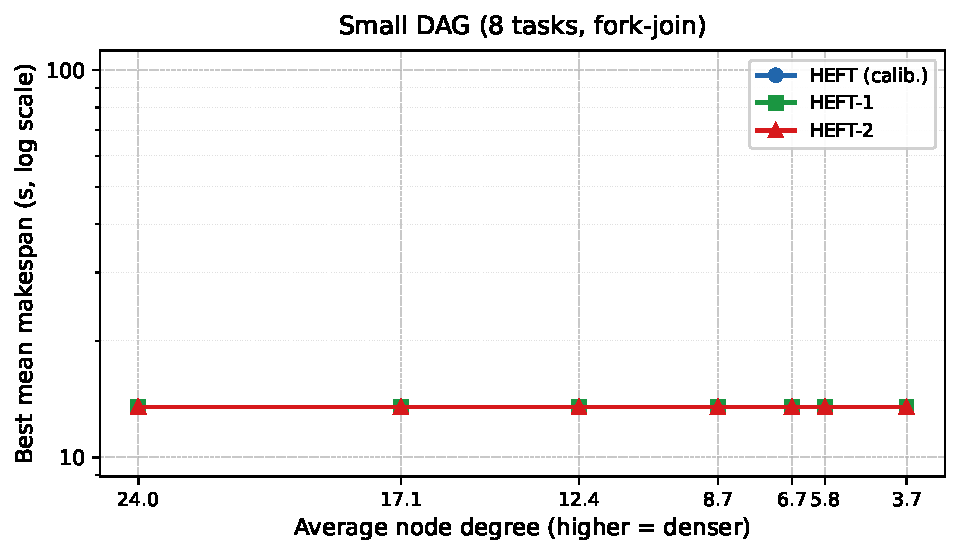
\includegraphics[width=0.85\textwidth]{noint_density_small.pdf}
\caption{No-interference: best-routing mean makespan vs.\ avg node degree --- Small DAG (8 tasks, fork-join). Error bars show 95\,\% CI over 30 seeds.}
\end{figure}

\begin{figure}[H]\centering
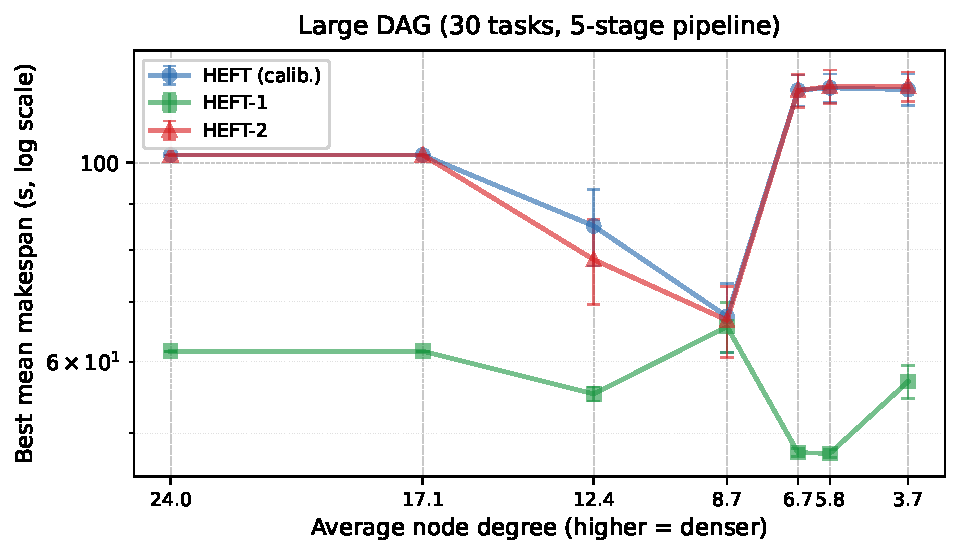
\includegraphics[width=0.85\textwidth]{noint_density_large.pdf}
\caption{No-interference: best-routing mean makespan vs.\ avg node degree --- Large DAG (30 tasks, 5-stage pipeline). Error bars show 95\,\% CI over 30 seeds.}
\end{figure}

\subsection{Additional Metrics vs.\ Density (Large DAG)}

Metrics are taken at the \emph{best} routing scheme for each scheduler at each density level, averaged over 30 seeds.

\begin{figure}[H]\centering
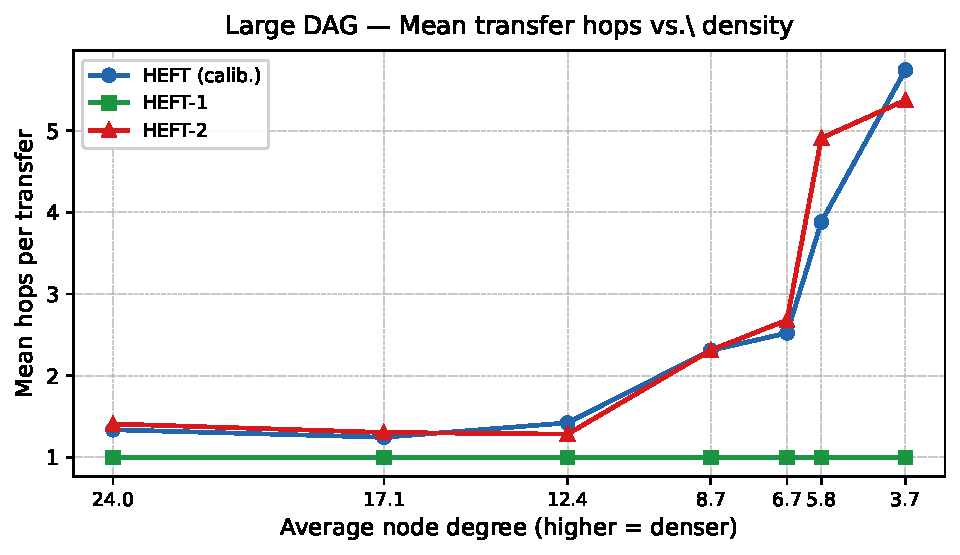
\includegraphics[width=0.85\textwidth]{noint_hops_large.pdf}
\caption{Mean hops per transfer for the best routing scheme at each density.}
\end{figure}

\begin{figure}[H]\centering
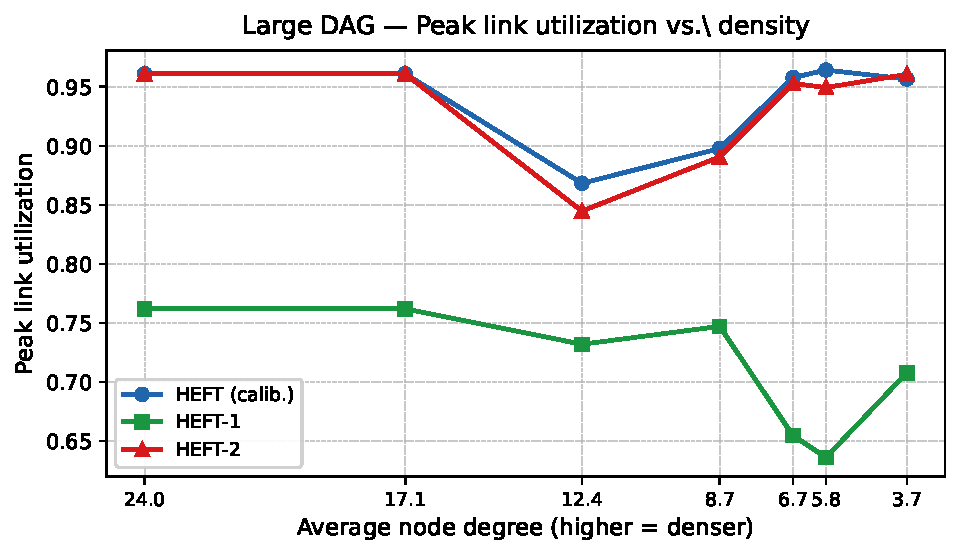
\includegraphics[width=0.85\textwidth]{noint_peaklu_large.pdf}
\caption{Peak link utilisation (max over all links) for the best routing scheme.}
\end{figure}

\begin{figure}[H]\centering
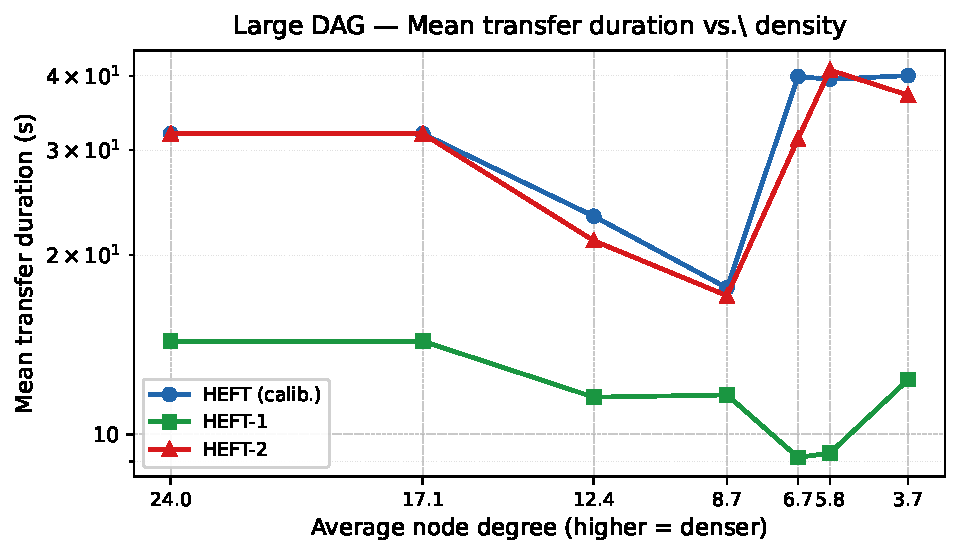
\includegraphics[width=0.85\textwidth]{noint_xferdur_large.pdf}
\caption{Mean transfer duration (s, log scale) for the best routing scheme.}
\end{figure}

\subsection{Best Routing Summary --- Small DAG (8 tasks)}

\begin{table}[H]\centering\small
\begin{tabular}{l r l r@{$\pm$}l r l r@{$\pm$}l r l r@{$\pm$}l r}
\toprule
\textbf{Density} & \textbf{Deg.} & \multicolumn{4}{c}{\textbf{HEFT}} & \multicolumn{4}{c}{\textbf{HEFT-1}} & \multicolumn{4}{c}{\textbf{HEFT-2}} \\
\cmidrule(lr){3-6}\cmidrule(lr){7-10}\cmidrule(lr){11-14}
& & \textbf{Rt} & \multicolumn{2}{c}{\textbf{ms(s)}} & \textbf{H} & \textbf{Rt} & \multicolumn{2}{c}{\textbf{ms(s)}} & \textbf{H} & \textbf{Rt} & \multicolumn{2}{c}{\textbf{ms(s)}} & \textbf{H} \\
\midrule
  L150 & 24.0 & W & \win{13.500} & 0.000 & 0.0 & W & \win{13.500} & 0.000 & 0.0 & W & \win{13.500} & 0.000 & 0.0 \\
  L200 & 17.1 & W & \win{13.500} & 0.000 & 0.0 & W & \win{13.500} & 0.000 & 0.0 & W & \win{13.500} & 0.000 & 0.0 \\
  L250 & 12.4 & W & \win{13.500} & 0.000 & 0.0 & W & \win{13.500} & 0.000 & 0.0 & W & \win{13.500} & 0.000 & 0.0 \\
  L300 & 8.7 & W & \win{13.500} & 0.000 & 0.0 & W & \win{13.500} & 0.000 & 0.0 & W & \win{13.500} & 0.000 & 0.0 \\
  L350 & 6.7 & W & \win{13.500} & 0.000 & 0.0 & W & \win{13.500} & 0.000 & 0.0 & W & \win{13.500} & 0.000 & 0.0 \\
  L400 & 5.8 & W & \win{13.500} & 0.000 & 0.0 & W & \win{13.500} & 0.000 & 0.0 & W & \win{13.500} & 0.000 & 0.0 \\
  L500 & 3.7 & W & \win{13.500} & 0.000 & 0.0 & W & \win{13.500} & 0.000 & 0.0 & W & \win{13.500} & 0.000 & 0.0 \\
\bottomrule\end{tabular}
\caption{Small DAG (8 tasks) --- best routing per (density, scheduler). ms = mean$\pm$95\,\%\,CI; H = mean hops. \win{Bold green}: overall best.}
\end{table}

\subsection{Best Routing Summary --- Large DAG (30 tasks)}

\begin{table}[H]\centering\small
\begin{tabular}{l r l r@{$\pm$}l r l r@{$\pm$}l r l r@{$\pm$}l r}
\toprule
\textbf{Density} & \textbf{Deg.} & \multicolumn{4}{c}{\textbf{HEFT}} & \multicolumn{4}{c}{\textbf{HEFT-1}} & \multicolumn{4}{c}{\textbf{HEFT-2}} \\
\cmidrule(lr){3-6}\cmidrule(lr){7-10}\cmidrule(lr){11-14}
& & \textbf{Rt} & \multicolumn{2}{c}{\textbf{ms(s)}} & \textbf{H} & \textbf{Rt} & \multicolumn{2}{c}{\textbf{ms(s)}} & \textbf{H} & \textbf{Rt} & \multicolumn{2}{c}{\textbf{ms(s)}} & \textbf{H} \\
\midrule
  L150 & 24.0 & W & 102.000 & 0.000 & 1.3 & W & 61.667 & 0.000 & 1.0 & W & 102.000 & 0.000 & 1.4 \\
  L200 & 17.1 & W & 102.000 & 0.000 & 1.2 & W & 61.667 & 0.000 & 1.0 & W & 102.000 & 0.000 & 1.3 \\
  L250 & 12.4 & GSD-D & 85.017 & 8.323 & 1.4 & GSD-D & 55.278 & 0.992 & 1.0 & GSD-D & 77.983 & 8.457 & 1.3 \\
  L300 & 8.7 & GSD-D & 67.394 & 5.958 & 2.3 & GSD & 65.667 & 4.227 & 1.0 & GSD-D & 66.767 & 6.055 & 2.3 \\
  L350 & 6.7 & S & 120.433 & 4.821 & 2.5 & GSD & 47.544 & 0.477 & 1.0 & GSD-D & 120.333 & 5.098 & 2.7 \\
  L400 & 5.8 & S & 121.133 & 4.407 & 3.9 & GSD-D & \win{47.458} & 0.485 & 1.0 & W & 121.600 & 5.206 & 4.9 \\
  L500 & 3.7 & S & 120.600 & 4.881 & 5.7 & GSD-D & 57.061 & 2.433 & 1.0 & GSD-D & 121.633 & 4.585 & 5.4 \\
\bottomrule\end{tabular}
\caption{Large DAG (30 tasks) --- best routing per (density, scheduler). ms = mean$\pm$95\,\%\,CI; H = mean hops. \win{Bold green}: overall best.}
\end{table}

\section{Full Random Network Results}

Mean$\pm$95\,\%\,CI makespan (s), mean hops, and peak link util over 30 seeds. \win{Bold green}: overall best for that density+DAG. \bad{Red}: worst in column.

\subsection{L150 (avg.\ degree 24.0) --- Small DAG (8 tasks)}
\begin{table}[H]\centering\small
\begin{tabular}{l r@{$\pm$}l r r r@{$\pm$}l r r r@{$\pm$}l r r}
\toprule
\textbf{Route} & \multicolumn{4}{c}{\textbf{HEFT}} & \multicolumn{4}{c}{\textbf{HEFT-1}} & \multicolumn{4}{c}{\textbf{HEFT-2}} \\
\cmidrule(lr){2-5}\cmidrule(lr){6-9}\cmidrule(lr){10-13}
& \multicolumn{2}{c}{\textbf{ms(s)}} & \textbf{H} & \textbf{PLU}& \multicolumn{2}{c}{\textbf{ms(s)}} & \textbf{H} & \textbf{PLU}& \multicolumn{2}{c}{\textbf{ms(s)}} & \textbf{H} & \textbf{PLU} \\
\midrule
  W & \win{13.500} & 0.000 & 0.0 & 0.000 & \win{13.500} & 0.000 & 0.0 & 0.000 & \win{13.500} & 0.000 & 0.0 & 0.000 \\
  S & \win{13.500} & 0.000 & 0.0 & 0.000 & \win{13.500} & 0.000 & 0.0 & 0.000 & \win{13.500} & 0.000 & 0.0 & 0.000 \\
  SH & \win{13.500} & 0.000 & 0.0 & 0.000 & \win{13.500} & 0.000 & 0.0 & 0.000 & \win{13.500} & 0.000 & 0.0 & 0.000 \\
  GO & \win{13.500} & 0.000 & 0.0 & 0.000 & \win{13.500} & 0.000 & 0.0 & 0.000 & \win{13.500} & 0.000 & 0.0 & 0.000 \\
  GS & \win{13.500} & 0.000 & 0.0 & 0.000 & \win{13.500} & 0.000 & 0.0 & 0.000 & \win{13.500} & 0.000 & 0.0 & 0.000 \\
  GSD & \win{13.500} & 0.000 & 0.0 & 0.000 & \win{13.500} & 0.000 & 0.0 & 0.000 & \win{13.500} & 0.000 & 0.0 & 0.000 \\
  GSD-D & \win{13.500} & 0.000 & 0.0 & 0.000 & \win{13.500} & 0.000 & 0.0 & 0.000 & \win{13.500} & 0.000 & 0.0 & 0.000 \\
\bottomrule\end{tabular}
\caption{L150 ($L=150$\,m) --- Small DAG (8 tasks). ms = mean$\pm$95\,\%\,CI; H = mean hops; PLU = peak link util.}
\end{table}

\subsection{L200 (avg.\ degree 17.1) --- Small DAG (8 tasks)}
\begin{table}[H]\centering\small
\begin{tabular}{l r@{$\pm$}l r r r@{$\pm$}l r r r@{$\pm$}l r r}
\toprule
\textbf{Route} & \multicolumn{4}{c}{\textbf{HEFT}} & \multicolumn{4}{c}{\textbf{HEFT-1}} & \multicolumn{4}{c}{\textbf{HEFT-2}} \\
\cmidrule(lr){2-5}\cmidrule(lr){6-9}\cmidrule(lr){10-13}
& \multicolumn{2}{c}{\textbf{ms(s)}} & \textbf{H} & \textbf{PLU}& \multicolumn{2}{c}{\textbf{ms(s)}} & \textbf{H} & \textbf{PLU}& \multicolumn{2}{c}{\textbf{ms(s)}} & \textbf{H} & \textbf{PLU} \\
\midrule
  W & \win{13.500} & 0.000 & 0.0 & 0.000 & \win{13.500} & 0.000 & 0.0 & 0.000 & \win{13.500} & 0.000 & 0.0 & 0.000 \\
  S & \win{13.500} & 0.000 & 0.0 & 0.000 & \win{13.500} & 0.000 & 0.0 & 0.000 & \win{13.500} & 0.000 & 0.0 & 0.000 \\
  SH & \win{13.500} & 0.000 & 0.0 & 0.000 & \win{13.500} & 0.000 & 0.0 & 0.000 & \win{13.500} & 0.000 & 0.0 & 0.000 \\
  GO & \win{13.500} & 0.000 & 0.0 & 0.000 & \win{13.500} & 0.000 & 0.0 & 0.000 & \win{13.500} & 0.000 & 0.0 & 0.000 \\
  GS & \win{13.500} & 0.000 & 0.0 & 0.000 & \win{13.500} & 0.000 & 0.0 & 0.000 & \win{13.500} & 0.000 & 0.0 & 0.000 \\
  GSD & \win{13.500} & 0.000 & 0.0 & 0.000 & \win{13.500} & 0.000 & 0.0 & 0.000 & \win{13.500} & 0.000 & 0.0 & 0.000 \\
  GSD-D & \win{13.500} & 0.000 & 0.0 & 0.000 & \win{13.500} & 0.000 & 0.0 & 0.000 & \win{13.500} & 0.000 & 0.0 & 0.000 \\
\bottomrule\end{tabular}
\caption{L200 ($L=200$\,m) --- Small DAG (8 tasks). ms = mean$\pm$95\,\%\,CI; H = mean hops; PLU = peak link util.}
\end{table}

\subsection{L250 (avg.\ degree 12.4) --- Small DAG (8 tasks)}
\begin{table}[H]\centering\small
\begin{tabular}{l r@{$\pm$}l r r r@{$\pm$}l r r r@{$\pm$}l r r}
\toprule
\textbf{Route} & \multicolumn{4}{c}{\textbf{HEFT}} & \multicolumn{4}{c}{\textbf{HEFT-1}} & \multicolumn{4}{c}{\textbf{HEFT-2}} \\
\cmidrule(lr){2-5}\cmidrule(lr){6-9}\cmidrule(lr){10-13}
& \multicolumn{2}{c}{\textbf{ms(s)}} & \textbf{H} & \textbf{PLU}& \multicolumn{2}{c}{\textbf{ms(s)}} & \textbf{H} & \textbf{PLU}& \multicolumn{2}{c}{\textbf{ms(s)}} & \textbf{H} & \textbf{PLU} \\
\midrule
  W & \win{13.500} & 0.000 & 0.0 & 0.000 & \win{13.500} & 0.000 & 0.0 & 0.000 & \win{13.500} & 0.000 & 0.0 & 0.000 \\
  S & \win{13.500} & 0.000 & 0.0 & 0.000 & \win{13.500} & 0.000 & 0.0 & 0.000 & \win{13.500} & 0.000 & 0.0 & 0.000 \\
  SH & \win{13.500} & 0.000 & 0.0 & 0.000 & \win{13.500} & 0.000 & 0.0 & 0.000 & \win{13.500} & 0.000 & 0.0 & 0.000 \\
  GO & \win{13.500} & 0.000 & 0.0 & 0.000 & \win{13.500} & 0.000 & 0.0 & 0.000 & \win{13.500} & 0.000 & 0.0 & 0.000 \\
  GS & \win{13.500} & 0.000 & 0.0 & 0.000 & \win{13.500} & 0.000 & 0.0 & 0.000 & \win{13.500} & 0.000 & 0.0 & 0.000 \\
  GSD & \win{13.500} & 0.000 & 0.0 & 0.000 & \win{13.500} & 0.000 & 0.0 & 0.000 & \win{13.500} & 0.000 & 0.0 & 0.000 \\
  GSD-D & \win{13.500} & 0.000 & 0.0 & 0.000 & \win{13.500} & 0.000 & 0.0 & 0.000 & \win{13.500} & 0.000 & 0.0 & 0.000 \\
\bottomrule\end{tabular}
\caption{L250 ($L=250$\,m) --- Small DAG (8 tasks). ms = mean$\pm$95\,\%\,CI; H = mean hops; PLU = peak link util.}
\end{table}

\subsection{L300 (avg.\ degree 8.7) --- Small DAG (8 tasks)}
\begin{table}[H]\centering\small
\begin{tabular}{l r@{$\pm$}l r r r@{$\pm$}l r r r@{$\pm$}l r r}
\toprule
\textbf{Route} & \multicolumn{4}{c}{\textbf{HEFT}} & \multicolumn{4}{c}{\textbf{HEFT-1}} & \multicolumn{4}{c}{\textbf{HEFT-2}} \\
\cmidrule(lr){2-5}\cmidrule(lr){6-9}\cmidrule(lr){10-13}
& \multicolumn{2}{c}{\textbf{ms(s)}} & \textbf{H} & \textbf{PLU}& \multicolumn{2}{c}{\textbf{ms(s)}} & \textbf{H} & \textbf{PLU}& \multicolumn{2}{c}{\textbf{ms(s)}} & \textbf{H} & \textbf{PLU} \\
\midrule
  W & \win{13.500} & 0.000 & 0.0 & 0.000 & \win{13.500} & 0.000 & 0.0 & 0.000 & \win{13.500} & 0.000 & 0.0 & 0.000 \\
  S & \win{13.500} & 0.000 & 0.0 & 0.000 & \win{13.500} & 0.000 & 0.0 & 0.000 & \win{13.500} & 0.000 & 0.0 & 0.000 \\
  SH & \win{13.500} & 0.000 & 0.0 & 0.000 & \win{13.500} & 0.000 & 0.0 & 0.000 & \win{13.500} & 0.000 & 0.0 & 0.000 \\
  GO & \win{13.500} & 0.000 & 0.0 & 0.000 & \win{13.500} & 0.000 & 0.0 & 0.000 & \win{13.500} & 0.000 & 0.0 & 0.000 \\
  GS & \win{13.500} & 0.000 & 0.0 & 0.000 & \win{13.500} & 0.000 & 0.0 & 0.000 & \win{13.500} & 0.000 & 0.0 & 0.000 \\
  GSD & \win{13.500} & 0.000 & 0.0 & 0.000 & \win{13.500} & 0.000 & 0.0 & 0.000 & \win{13.500} & 0.000 & 0.0 & 0.000 \\
  GSD-D & \win{13.500} & 0.000 & 0.0 & 0.000 & \win{13.500} & 0.000 & 0.0 & 0.000 & \win{13.500} & 0.000 & 0.0 & 0.000 \\
\bottomrule\end{tabular}
\caption{L300 ($L=300$\,m) --- Small DAG (8 tasks). ms = mean$\pm$95\,\%\,CI; H = mean hops; PLU = peak link util.}
\end{table}

\subsection{L350 (avg.\ degree 6.7) --- Small DAG (8 tasks)}
\begin{table}[H]\centering\small
\begin{tabular}{l r@{$\pm$}l r r r@{$\pm$}l r r r@{$\pm$}l r r}
\toprule
\textbf{Route} & \multicolumn{4}{c}{\textbf{HEFT}} & \multicolumn{4}{c}{\textbf{HEFT-1}} & \multicolumn{4}{c}{\textbf{HEFT-2}} \\
\cmidrule(lr){2-5}\cmidrule(lr){6-9}\cmidrule(lr){10-13}
& \multicolumn{2}{c}{\textbf{ms(s)}} & \textbf{H} & \textbf{PLU}& \multicolumn{2}{c}{\textbf{ms(s)}} & \textbf{H} & \textbf{PLU}& \multicolumn{2}{c}{\textbf{ms(s)}} & \textbf{H} & \textbf{PLU} \\
\midrule
  W & \win{13.500} & 0.000 & 0.0 & 0.000 & \win{13.500} & 0.000 & 0.0 & 0.000 & \win{13.500} & 0.000 & 0.0 & 0.000 \\
  S & \win{13.500} & 0.000 & 0.0 & 0.000 & \win{13.500} & 0.000 & 0.0 & 0.000 & \win{13.500} & 0.000 & 0.0 & 0.000 \\
  SH & \win{13.500} & 0.000 & 0.0 & 0.000 & \win{13.500} & 0.000 & 0.0 & 0.000 & \win{13.500} & 0.000 & 0.0 & 0.000 \\
  GO & \win{13.500} & 0.000 & 0.0 & 0.000 & \win{13.500} & 0.000 & 0.0 & 0.000 & \win{13.500} & 0.000 & 0.0 & 0.000 \\
  GS & \win{13.500} & 0.000 & 0.0 & 0.000 & \win{13.500} & 0.000 & 0.0 & 0.000 & \win{13.500} & 0.000 & 0.0 & 0.000 \\
  GSD & \win{13.500} & 0.000 & 0.0 & 0.000 & \win{13.500} & 0.000 & 0.0 & 0.000 & \win{13.500} & 0.000 & 0.0 & 0.000 \\
  GSD-D & \win{13.500} & 0.000 & 0.0 & 0.000 & \win{13.500} & 0.000 & 0.0 & 0.000 & \win{13.500} & 0.000 & 0.0 & 0.000 \\
\bottomrule\end{tabular}
\caption{L350 ($L=350$\,m) --- Small DAG (8 tasks). ms = mean$\pm$95\,\%\,CI; H = mean hops; PLU = peak link util.}
\end{table}

\subsection{L400 (avg.\ degree 5.8) --- Small DAG (8 tasks)}
\begin{table}[H]\centering\small
\begin{tabular}{l r@{$\pm$}l r r r@{$\pm$}l r r r@{$\pm$}l r r}
\toprule
\textbf{Route} & \multicolumn{4}{c}{\textbf{HEFT}} & \multicolumn{4}{c}{\textbf{HEFT-1}} & \multicolumn{4}{c}{\textbf{HEFT-2}} \\
\cmidrule(lr){2-5}\cmidrule(lr){6-9}\cmidrule(lr){10-13}
& \multicolumn{2}{c}{\textbf{ms(s)}} & \textbf{H} & \textbf{PLU}& \multicolumn{2}{c}{\textbf{ms(s)}} & \textbf{H} & \textbf{PLU}& \multicolumn{2}{c}{\textbf{ms(s)}} & \textbf{H} & \textbf{PLU} \\
\midrule
  W & \win{13.500} & 0.000 & 0.0 & 0.000 & \win{13.500} & 0.000 & 0.0 & 0.000 & \win{13.500} & 0.000 & 0.0 & 0.000 \\
  S & \win{13.500} & 0.000 & 0.0 & 0.000 & \win{13.500} & 0.000 & 0.0 & 0.000 & \win{13.500} & 0.000 & 0.0 & 0.000 \\
  SH & \win{13.500} & 0.000 & 0.0 & 0.000 & \win{13.500} & 0.000 & 0.0 & 0.000 & \win{13.500} & 0.000 & 0.0 & 0.000 \\
  GO & \win{13.500} & 0.000 & 0.0 & 0.000 & \win{13.500} & 0.000 & 0.0 & 0.000 & \win{13.500} & 0.000 & 0.0 & 0.000 \\
  GS & \win{13.500} & 0.000 & 0.0 & 0.000 & \win{13.500} & 0.000 & 0.0 & 0.000 & \win{13.500} & 0.000 & 0.0 & 0.000 \\
  GSD & \win{13.500} & 0.000 & 0.0 & 0.000 & \win{13.500} & 0.000 & 0.0 & 0.000 & \win{13.500} & 0.000 & 0.0 & 0.000 \\
  GSD-D & \win{13.500} & 0.000 & 0.0 & 0.000 & \win{13.500} & 0.000 & 0.0 & 0.000 & \win{13.500} & 0.000 & 0.0 & 0.000 \\
\bottomrule\end{tabular}
\caption{L400 ($L=400$\,m) --- Small DAG (8 tasks). ms = mean$\pm$95\,\%\,CI; H = mean hops; PLU = peak link util.}
\end{table}

\subsection{L500 (avg.\ degree 3.7) --- Small DAG (8 tasks)}
\begin{table}[H]\centering\small
\begin{tabular}{l r@{$\pm$}l r r r@{$\pm$}l r r r@{$\pm$}l r r}
\toprule
\textbf{Route} & \multicolumn{4}{c}{\textbf{HEFT}} & \multicolumn{4}{c}{\textbf{HEFT-1}} & \multicolumn{4}{c}{\textbf{HEFT-2}} \\
\cmidrule(lr){2-5}\cmidrule(lr){6-9}\cmidrule(lr){10-13}
& \multicolumn{2}{c}{\textbf{ms(s)}} & \textbf{H} & \textbf{PLU}& \multicolumn{2}{c}{\textbf{ms(s)}} & \textbf{H} & \textbf{PLU}& \multicolumn{2}{c}{\textbf{ms(s)}} & \textbf{H} & \textbf{PLU} \\
\midrule
  W & \win{13.500} & 0.000 & 0.0 & 0.000 & \win{13.500} & 0.000 & 0.0 & 0.000 & \win{13.500} & 0.000 & 0.0 & 0.000 \\
  S & \win{13.500} & 0.000 & 0.0 & 0.000 & \win{13.500} & 0.000 & 0.0 & 0.000 & \win{13.500} & 0.000 & 0.0 & 0.000 \\
  SH & \win{13.500} & 0.000 & 0.0 & 0.000 & \win{13.500} & 0.000 & 0.0 & 0.000 & \win{13.500} & 0.000 & 0.0 & 0.000 \\
  GO & \win{13.500} & 0.000 & 0.0 & 0.000 & \win{13.500} & 0.000 & 0.0 & 0.000 & \win{13.500} & 0.000 & 0.0 & 0.000 \\
  GS & \win{13.500} & 0.000 & 0.0 & 0.000 & \win{13.500} & 0.000 & 0.0 & 0.000 & \win{13.500} & 0.000 & 0.0 & 0.000 \\
  GSD & \win{13.500} & 0.000 & 0.0 & 0.000 & \win{13.500} & 0.000 & 0.0 & 0.000 & \win{13.500} & 0.000 & 0.0 & 0.000 \\
  GSD-D & \win{13.500} & 0.000 & 0.0 & 0.000 & \win{13.500} & 0.000 & 0.0 & 0.000 & \win{13.500} & 0.000 & 0.0 & 0.000 \\
\bottomrule\end{tabular}
\caption{L500 ($L=500$\,m) --- Small DAG (8 tasks). ms = mean$\pm$95\,\%\,CI; H = mean hops; PLU = peak link util.}
\end{table}

\subsection{L150 (avg.\ degree 24.0) --- Large DAG (30 tasks)}
\begin{table}[H]\centering\small
\begin{tabular}{l r@{$\pm$}l r r r@{$\pm$}l r r r@{$\pm$}l r r}
\toprule
\textbf{Route} & \multicolumn{4}{c}{\textbf{HEFT}} & \multicolumn{4}{c}{\textbf{HEFT-1}} & \multicolumn{4}{c}{\textbf{HEFT-2}} \\
\cmidrule(lr){2-5}\cmidrule(lr){6-9}\cmidrule(lr){10-13}
& \multicolumn{2}{c}{\textbf{ms(s)}} & \textbf{H} & \textbf{PLU}& \multicolumn{2}{c}{\textbf{ms(s)}} & \textbf{H} & \textbf{PLU}& \multicolumn{2}{c}{\textbf{ms(s)}} & \textbf{H} & \textbf{PLU} \\
\midrule
  W & 102.000 & 0.000 & 1.3 & 0.961 & \win{61.667} & 0.000 & 1.0 & 0.762 & 102.000 & 0.000 & 1.4 & 0.961 \\
  S & 102.000 & 0.000 & 1.3 & 0.961 & \win{61.667} & 0.000 & 1.0 & 0.762 & 102.000 & 0.000 & 1.3 & 0.961 \\
  SH & 102.000 & 0.000 & 1.4 & 0.961 & \win{61.667} & 0.000 & 1.0 & 0.762 & 102.000 & 0.000 & 1.2 & 0.961 \\
  GO & \bad{107.000} & 0.000 & 4.0 & 0.963 & \win{61.667} & 0.000 & 4.0 & 0.762 & \bad{107.000} & 0.000 & 4.0 & 0.963 \\
  GS & \bad{107.000} & 0.000 & 4.0 & 0.963 & \win{61.667} & 0.000 & 4.0 & 0.762 & \bad{107.000} & 0.000 & 4.0 & 0.963 \\
  GSD & \bad{107.000} & 0.000 & 1.3 & 0.963 & \win{61.667} & 0.000 & 1.0 & 0.762 & \bad{107.000} & 0.000 & 1.4 & 0.963 \\
  GSD-D & \bad{107.000} & 0.000 & 1.3 & 0.963 & \win{61.667} & 0.000 & 1.0 & 0.762 & \bad{107.000} & 0.000 & 1.2 & 0.963 \\
\bottomrule\end{tabular}
\caption{L150 ($L=150$\,m) --- Large DAG (30 tasks). ms = mean$\pm$95\,\%\,CI; H = mean hops; PLU = peak link util.}
\end{table}

\subsection{L200 (avg.\ degree 17.1) --- Large DAG (30 tasks)}
\begin{table}[H]\centering\small
\begin{tabular}{l r@{$\pm$}l r r r@{$\pm$}l r r r@{$\pm$}l r r}
\toprule
\textbf{Route} & \multicolumn{4}{c}{\textbf{HEFT}} & \multicolumn{4}{c}{\textbf{HEFT-1}} & \multicolumn{4}{c}{\textbf{HEFT-2}} \\
\cmidrule(lr){2-5}\cmidrule(lr){6-9}\cmidrule(lr){10-13}
& \multicolumn{2}{c}{\textbf{ms(s)}} & \textbf{H} & \textbf{PLU}& \multicolumn{2}{c}{\textbf{ms(s)}} & \textbf{H} & \textbf{PLU}& \multicolumn{2}{c}{\textbf{ms(s)}} & \textbf{H} & \textbf{PLU} \\
\midrule
  W & 102.000 & 0.000 & 1.2 & 0.961 & \win{61.667} & 0.000 & 1.0 & 0.762 & 102.000 & 0.000 & 1.3 & 0.961 \\
  S & 102.000 & 0.000 & 1.3 & 0.961 & \win{61.667} & 0.000 & 1.0 & 0.762 & 102.000 & 0.000 & 1.3 & 0.961 \\
  SH & 102.000 & 0.000 & 1.4 & 0.961 & \win{61.667} & 0.000 & 1.0 & 0.762 & 102.000 & 0.000 & 1.4 & 0.961 \\
  GO & \bad{107.000} & 0.000 & 4.0 & 0.963 & \win{61.667} & 0.000 & 4.0 & 0.762 & \bad{107.000} & 0.000 & 4.0 & 0.963 \\
  GS & \bad{107.000} & 0.000 & 4.0 & 0.963 & \win{61.667} & 0.000 & 4.0 & 0.762 & \bad{107.000} & 0.000 & 4.0 & 0.963 \\
  GSD & \bad{107.000} & 0.000 & 1.4 & 0.963 & \win{61.667} & 0.000 & 1.0 & 0.762 & \bad{107.000} & 0.000 & 1.3 & 0.963 \\
  GSD-D & \bad{107.000} & 0.000 & 1.3 & 0.963 & \win{61.667} & 0.000 & 1.0 & 0.762 & \bad{107.000} & 0.000 & 1.3 & 0.963 \\
\bottomrule\end{tabular}
\caption{L200 ($L=200$\,m) --- Large DAG (30 tasks). ms = mean$\pm$95\,\%\,CI; H = mean hops; PLU = peak link util.}
\end{table}

\subsection{L250 (avg.\ degree 12.4) --- Large DAG (30 tasks)}
\begin{table}[H]\centering\small
\begin{tabular}{l r@{$\pm$}l r r r@{$\pm$}l r r r@{$\pm$}l r r}
\toprule
\textbf{Route} & \multicolumn{4}{c}{\textbf{HEFT}} & \multicolumn{4}{c}{\textbf{HEFT-1}} & \multicolumn{4}{c}{\textbf{HEFT-2}} \\
\cmidrule(lr){2-5}\cmidrule(lr){6-9}\cmidrule(lr){10-13}
& \multicolumn{2}{c}{\textbf{ms(s)}} & \textbf{H} & \textbf{PLU}& \multicolumn{2}{c}{\textbf{ms(s)}} & \textbf{H} & \textbf{PLU}& \multicolumn{2}{c}{\textbf{ms(s)}} & \textbf{H} & \textbf{PLU} \\
\midrule
  W & 122.300 & 4.801 & 1.3 & 0.956 & \bad{61.667} & 0.000 & 1.0 & 0.762 & 125.100 & 4.568 & 1.4 & 0.953 \\
  S & 124.267 & 4.357 & 1.3 & 0.959 & \bad{61.667} & 0.000 & 1.0 & 0.762 & 122.967 & 4.994 & 1.4 & 0.951 \\
  SH & \bad{127.467} & 4.349 & 1.5 & 0.947 & \bad{61.667} & 0.000 & 1.0 & 0.762 & \bad{128.000} & 3.669 & 1.4 & 0.955 \\
  GO & 105.000 & 0.930 & 4.0 & 0.962 & \bad{61.667} & 0.000 & 4.0 & 0.762 & 103.833 & 0.915 & 4.0 & 0.962 \\
  GS & 105.000 & 0.930 & 4.0 & 0.962 & \bad{61.667} & 0.000 & 4.0 & 0.762 & 103.667 & 0.895 & 4.0 & 0.962 \\
  GSD & 88.300 & 7.906 & 1.3 & 0.882 & 55.722 & 0.866 & 1.0 & 0.758 & 80.083 & 8.802 & 1.3 & 0.847 \\
  GSD-D & 85.017 & 8.323 & 1.4 & 0.868 & \win{55.278} & 0.992 & 1.0 & 0.732 & 77.983 & 8.457 & 1.3 & 0.845 \\
\bottomrule\end{tabular}
\caption{L250 ($L=250$\,m) --- Large DAG (30 tasks). ms = mean$\pm$95\,\%\,CI; H = mean hops; PLU = peak link util.}
\end{table}

\subsection{L300 (avg.\ degree 8.7) --- Large DAG (30 tasks)}
\begin{table}[H]\centering\small
\begin{tabular}{l r@{$\pm$}l r r r@{$\pm$}l r r r@{$\pm$}l r r}
\toprule
\textbf{Route} & \multicolumn{4}{c}{\textbf{HEFT}} & \multicolumn{4}{c}{\textbf{HEFT-1}} & \multicolumn{4}{c}{\textbf{HEFT-2}} \\
\cmidrule(lr){2-5}\cmidrule(lr){6-9}\cmidrule(lr){10-13}
& \multicolumn{2}{c}{\textbf{ms(s)}} & \textbf{H} & \textbf{PLU}& \multicolumn{2}{c}{\textbf{ms(s)}} & \textbf{H} & \textbf{PLU}& \multicolumn{2}{c}{\textbf{ms(s)}} & \textbf{H} & \textbf{PLU} \\
\midrule
  W & 127.900 & 4.053 & 2.4 & 0.950 & 71.828 & 7.439 & 1.0 & 0.771 & 123.067 & 4.703 & 2.3 & 0.956 \\
  S & 121.867 & 4.984 & 2.3 & 0.953 & 68.037 & 6.820 & 1.0 & 0.751 & 122.133 & 4.749 & 2.3 & 0.957 \\
  SH & \bad{128.500} & 3.751 & 2.4 & 0.951 & \bad{77.074} & 7.720 & 1.0 & 0.800 & \bad{124.933} & 4.528 & 2.4 & 0.954 \\
  GO & 102.833 & 0.708 & 3.8 & 0.961 & 72.382 & 8.433 & 3.1 & 0.775 & 103.000 & 0.759 & 3.8 & 0.961 \\
  GS & 102.500 & 0.570 & 3.8 & 0.961 & 71.838 & 6.305 & 2.7 & 0.815 & 102.500 & 0.570 & 3.7 & 0.961 \\
  GSD & 67.472 & 6.607 & 2.4 & 0.894 & \win{65.667} & 4.227 & 1.0 & 0.747 & 68.117 & 6.513 & 2.3 & 0.901 \\
  GSD-D & 67.394 & 5.958 & 2.3 & 0.898 & 66.521 & 4.218 & 1.0 & 0.755 & 66.767 & 6.055 & 2.3 & 0.891 \\
\bottomrule\end{tabular}
\caption{L300 ($L=300$\,m) --- Large DAG (30 tasks). ms = mean$\pm$95\,\%\,CI; H = mean hops; PLU = peak link util.}
\end{table}

\subsection{L350 (avg.\ degree 6.7) --- Large DAG (30 tasks)}
\begin{table}[H]\centering\small
\begin{tabular}{l r@{$\pm$}l r r r@{$\pm$}l r r r@{$\pm$}l r r}
\toprule
\textbf{Route} & \multicolumn{4}{c}{\textbf{HEFT}} & \multicolumn{4}{c}{\textbf{HEFT-1}} & \multicolumn{4}{c}{\textbf{HEFT-2}} \\
\cmidrule(lr){2-5}\cmidrule(lr){6-9}\cmidrule(lr){10-13}
& \multicolumn{2}{c}{\textbf{ms(s)}} & \textbf{H} & \textbf{PLU}& \multicolumn{2}{c}{\textbf{ms(s)}} & \textbf{H} & \textbf{PLU}& \multicolumn{2}{c}{\textbf{ms(s)}} & \textbf{H} & \textbf{PLU} \\
\midrule
  W & \bad{128.000} & 3.669 & 2.7 & 0.955 & 61.578 & 0.656 & 1.0 & 0.705 & 121.200 & 4.768 & 2.5 & 0.958 \\
  S & 120.433 & 4.821 & 2.5 & 0.958 & \bad{62.114} & 0.551 & 1.0 & 0.686 & 122.300 & 4.801 & 2.6 & 0.956 \\
  SH & 124.167 & 4.674 & 2.7 & 0.954 & \bad{62.067} & 0.469 & 1.0 & 0.712 & \bad{126.800} & 4.229 & 2.8 & 0.952 \\
  GO & 123.567 & 4.842 & 3.0 & 0.952 & 60.430 & 0.738 & 2.4 & 0.715 & 125.267 & 4.606 & 3.1 & 0.952 \\
  GS & 121.200 & 4.768 & 2.9 & 0.958 & 61.285 & 0.702 & 2.7 & 0.708 & 125.100 & 4.568 & 3.1 & 0.953 \\
  GSD & 123.067 & 4.703 & 2.6 & 0.956 & \win{47.544} & 0.477 & 1.0 & 0.654 & 121.967 & 4.696 & 2.5 & 0.958 \\
  GSD-D & 122.467 & 4.851 & 2.7 & 0.955 & 47.718 & 0.454 & 1.0 & 0.643 & 120.333 & 5.098 & 2.7 & 0.953 \\
\bottomrule\end{tabular}
\caption{L350 ($L=350$\,m) --- Large DAG (30 tasks). ms = mean$\pm$95\,\%\,CI; H = mean hops; PLU = peak link util.}
\end{table}

\subsection{L400 (avg.\ degree 5.8) --- Large DAG (30 tasks)}
\begin{table}[H]\centering\small
\begin{tabular}{l r@{$\pm$}l r r r@{$\pm$}l r r r@{$\pm$}l r r}
\toprule
\textbf{Route} & \multicolumn{4}{c}{\textbf{HEFT}} & \multicolumn{4}{c}{\textbf{HEFT-1}} & \multicolumn{4}{c}{\textbf{HEFT-2}} \\
\cmidrule(lr){2-5}\cmidrule(lr){6-9}\cmidrule(lr){10-13}
& \multicolumn{2}{c}{\textbf{ms(s)}} & \textbf{H} & \textbf{PLU}& \multicolumn{2}{c}{\textbf{ms(s)}} & \textbf{H} & \textbf{PLU}& \multicolumn{2}{c}{\textbf{ms(s)}} & \textbf{H} & \textbf{PLU} \\
\midrule
  W & \bad{126.467} & 4.162 & 4.7 & 0.954 & 60.967 & 0.772 & 1.0 & 0.696 & 121.600 & 5.206 & 4.9 & 0.949 \\
  S & 121.133 & 4.407 & 3.9 & 0.964 & 61.456 & 0.687 & 1.0 & 0.703 & 122.733 & 4.604 & 4.4 & 0.958 \\
  SH & 123.400 & 4.797 & 4.5 & 0.954 & 61.138 & 0.717 & 1.0 & 0.710 & 124.933 & 4.528 & 5.1 & 0.954 \\
  GO & 125.867 & 4.396 & 4.9 & 0.953 & 60.942 & 0.765 & 2.3 & 0.699 & 125.700 & 4.359 & 4.9 & 0.954 \\
  GS & 124.333 & 4.716 & 5.2 & 0.953 & \bad{61.602} & 0.661 & 2.7 & 0.702 & \bad{126.467} & 4.162 & 4.8 & 0.954 \\
  GSD & 125.367 & 4.281 & 4.7 & 0.957 & 47.544 & 0.477 & 1.0 & 0.630 & 123.067 & 4.703 & 4.6 & 0.956 \\
  GSD-D & 122.300 & 4.801 & 4.6 & 0.956 & \win{47.458} & 0.485 & 1.0 & 0.636 & 125.700 & 4.359 & 4.8 & 0.954 \\
\bottomrule\end{tabular}
\caption{L400 ($L=400$\,m) --- Large DAG (30 tasks). ms = mean$\pm$95\,\%\,CI; H = mean hops; PLU = peak link util.}
\end{table}

\subsection{L500 (avg.\ degree 3.7) --- Large DAG (30 tasks)}
\begin{table}[H]\centering\small
\begin{tabular}{l r@{$\pm$}l r r r@{$\pm$}l r r r@{$\pm$}l r r}
\toprule
\textbf{Route} & \multicolumn{4}{c}{\textbf{HEFT}} & \multicolumn{4}{c}{\textbf{HEFT-1}} & \multicolumn{4}{c}{\textbf{HEFT-2}} \\
\cmidrule(lr){2-5}\cmidrule(lr){6-9}\cmidrule(lr){10-13}
& \multicolumn{2}{c}{\textbf{ms(s)}} & \textbf{H} & \textbf{PLU}& \multicolumn{2}{c}{\textbf{ms(s)}} & \textbf{H} & \textbf{PLU}& \multicolumn{2}{c}{\textbf{ms(s)}} & \textbf{H} & \textbf{PLU} \\
\midrule
  W & 122.133 & 4.749 & 5.9 & 0.957 & 61.194 & 0.751 & 1.0 & 0.719 & 124.933 & 4.528 & 6.3 & 0.954 \\
  S & 120.600 & 4.881 & 5.7 & 0.957 & 60.833 & 0.906 & 1.0 & 0.691 & 124.600 & 4.445 & 5.9 & 0.956 \\
  SH & 121.200 & 4.768 & 5.7 & 0.958 & 60.683 & 0.853 & 1.0 & 0.702 & \bad{129.000} & 3.823 & 6.7 & 0.948 \\
  GO & 124.500 & 4.757 & 6.5 & 0.951 & 61.100 & 0.835 & 1.7 & 0.704 & 126.033 & 4.431 & 6.0 & 0.952 \\
  GS & 124.600 & 4.445 & 6.0 & 0.956 & \bad{61.567} & 0.799 & 1.7 & 0.702 & 126.733 & 3.831 & 5.6 & 0.958 \\
  GSD & 123.833 & 4.585 & 5.5 & 0.956 & 58.050 & 2.002 & 1.0 & 0.701 & 124.933 & 4.528 & 5.9 & 0.954 \\
  GSD-D & \bad{125.533} & 4.321 & 6.1 & 0.955 & \win{57.061} & 2.433 & 1.0 & 0.708 & 121.633 & 4.585 & 5.4 & 0.961 \\
\bottomrule\end{tabular}
\caption{L500 ($L=500$\,m) --- Large DAG (30 tasks). ms = mean$\pm$95\,\%\,CI; H = mean hops; PLU = peak link util.}
\end{table}

\section{Analysis}

\subsection{Small DAG: Compute-Bound, All Metrics Trivial}

All routing schemes and schedulers produce identical makespan (13.500\,s) on the small DAG across both grid sizes and all density levels. Transfers are same-node (0 hops, 0 link utilisation) because HEFT-1 co-locates all 8 tasks. Even under HEFT/HEFT-2, the DAG's compute time dominates: transfer costs are negligible without interference.

\subsection{Why GSD/GSD-D Win on the Large DAG}

The extra metrics reveal the mechanism clearly. On the $7\times7$ grid large DAG under HEFT-1:

\begin{center}\small
\begin{tabular}{l r r r r}\toprule
\textbf{Routing} & \textbf{Makespan (s)} & \textbf{Mean hops} & \textbf{Peak link util.} & \textbf{Mean xfer dur.\ (s)} \\\midrule
  W & 141.357 & 1.0 & 0.933 & 27.7 \\
  S & 142.690 & 1.0 & 0.933 & 28.4 \\
  SH & 134.690 & 1.0 & 0.929 & 25.0 \\
  GS & 147.193 & 2.4 & 0.927 & 31.5 \\
  GO & 145.357 & 2.4 & 0.935 & 29.0 \\
  GSD & 71.483 & 1.0 & 0.786 & 13.7 \\
  GSD-D & 72.417 & 1.0 & 0.773 & 13.8 \\
\bottomrule\end{tabular}
\end{center}

W, S, and SH all use 1-hop paths but achieve peak link utilisation of 0.93, with mean transfer durations of 25--28\,s. GS and GO use 2.4--2.7 hops on average. GSD and GSD-D also use 1-hop paths but reduce peak link utilisation to 0.77--0.79 and halve the mean transfer duration to 13.7\,s, directly explaining the $2\times$ makespan advantage.

\subsection{Comparison to csma\_bianchi Results}

Removing interference collapses the large-DAG makespan from 150--927\,s (csma\_bianchi, best routing) to 47--66\,s (no interference, best routing) under HEFT-1---a $3$--$14\times$ reduction. This confirms that the dominant cost in the csma\_bianchi experiments was inter-link spectrum contention, not intra-link queuing.

\subsection{Reproducing These Results}
\begin{verbatim}
cd ncsim/
python run_no_interference_eval.py      # ~70 min (12 060 runs)
python compute_noint_augmented.py       # reads existing traces
python gen_no_interference_report.py    # regenerates tex + plots
cd docs/ && pdflatex no_interference_results.tex
\end{verbatim}

\end{document}